\documentclass[12pt,a4paper,openany]{book}
\usepackage[french,UKenglish]{babel}
\usepackage[utf8]{inputenc}
\usepackage[T1]{fontenc}
\usepackage[a4paper,left=2cm,top=3cm,right=2cm,bottom=2.5cm]{geometry}
\usepackage{amsmath, amsfonts, amssymb}
\usepackage{mathrsfs}
\usepackage[pdftex]{graphicx}
\usepackage{ragged2e}
\usepackage{setspace}
\usepackage{multirow}
\usepackage[T1]{fontenc} %para escurecer a cor da fonte
\usepackage{lmodern}
\usepackage[mathcal]{eucal}
\usepackage{pdfpages}
\usepackage{latexsym}
\usepackage{multicol}
\usepackage{minitoc}
\usepackage{pdftexcmds}
\usepackage{tikz}
\usepackage{subfigure}
\usepackage[version=3]{mhchem}
\usepackage{bm}
\usepackage{booktabs}
\usepackage[all]{xy}
\usepackage{makeidx}
\usepackage{float}
\usepackage{geometry}
\usepackage{longtable}
\usepackage{caption}
\usepackage[para,online,flushleft]{threeparttable}
\usepackage[multiple]{footmisc} %permite colocar virgulas entre footnotes
\usepackage{relsize} %permite aumentar o tamanho das integrais
\usepackage{pbox} %permite quebrar a linha numa tabela
\usepackage{paralist}
\usepackage[toc,page]{appendix}
\bibliographystyle{unsrt}
\sloppy



\begin{document}
	
	\textbf{Tetracene}
	
	\begin{figure}[h]
		\centering
		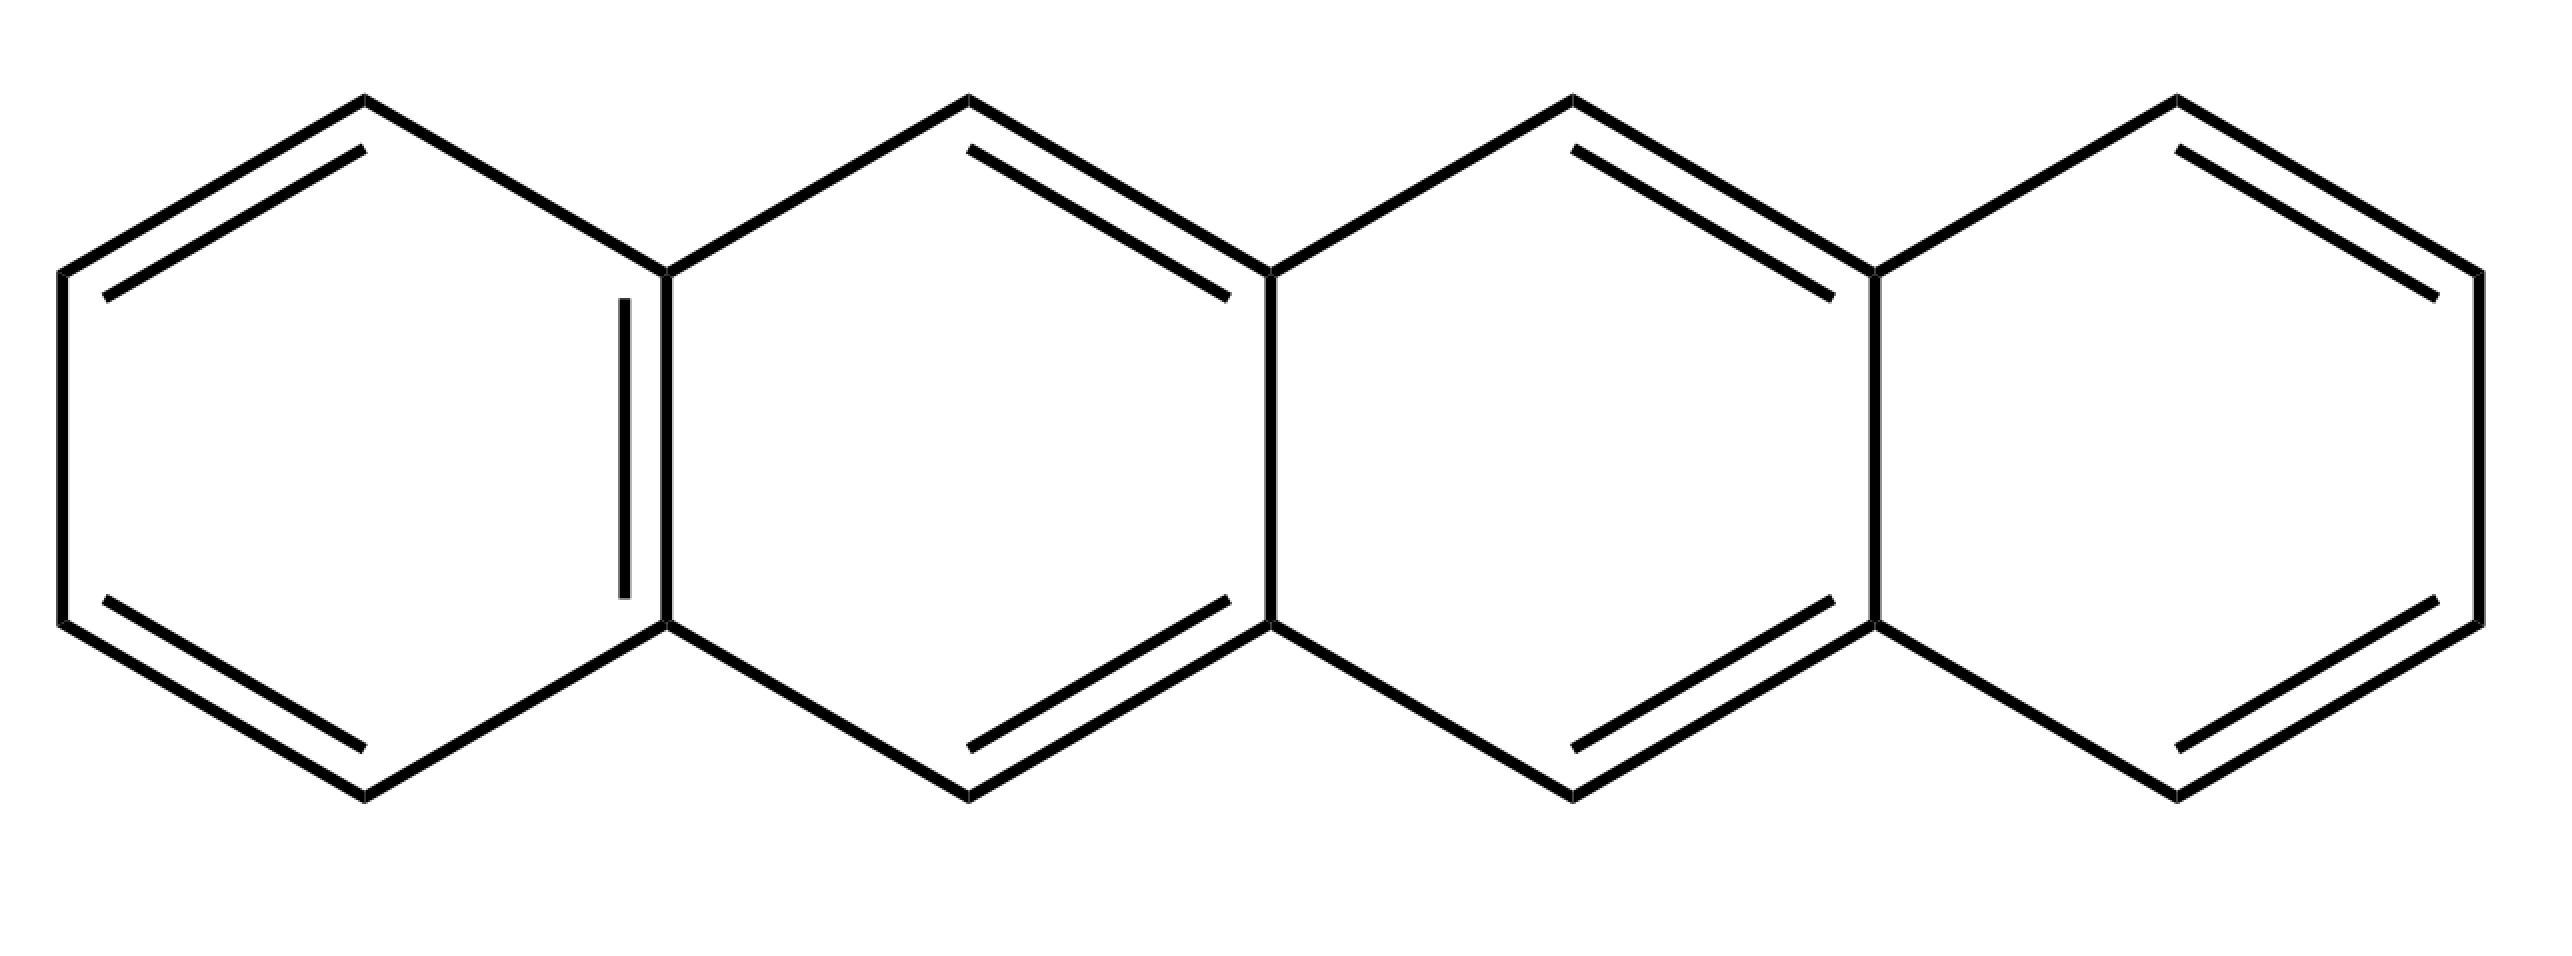
\includegraphics[scale=0.2]{tetracene}
		\caption{Tetracene molecule}
	\end{figure} 
 
 
 	\begin{table}[t]
 		\caption{Lattice parameters of Tetracene molecule calculated in VASP code} \label{table13}
 		\begin{center}
 			\begin{threeparttable}
 				\begin{tabular}{c c c c c c c}
 					\toprule
 					& \textbf{D2} & \textbf{D3} & \textbf{TS} & \textbf{TS-SCS} & \textbf{PBE*} & \textbf{Exp} \\
 					\midrule
 					\textbf{a} &7.54 (7.41) &  7.92 & 7.71 & 7.70 & 9.25 & 7.90\\
 					\textbf{b}& 5.96 (5.83) & 6.00 & 5.99 & 6.08 & 7.21 & 6.03 \\
 					\textbf{c}& 13.28 (13.39) & 13.38 & 13.38 & 13.47 & 16.62 & 13.53 \\
 					\textbf{$\alpha$} & 102.10 (102.21) & 101.21 & 101.36 & 100.97 & 101.36 &100.30\\
 					\textbf{$\beta$} & 114.33 (113.23) & 113.26 & 113.61 & 114.39 & 112.14 & 113.20\\
 					\textbf{$\gamma$} &85.20 (85.11) & 85.89 & 85.74 & 85.68 & 86.67 & 86.30\\
 					\textbf{Volume ($\AA^{3}$)} & 531.41 (519.01) & 572.96 & 554.74 &  563.74 & 1007.16 & 582.85\\
 					\bottomrule
 				\end{tabular} 
 				
 				\begin{tablenotes}
 					\item[*] without dispersion correction
 					\item[()] Parenthesis values were calculated with CRYSTAL program
 					\item[Exp] Campbell, R. B \textit{et al} Acta cryst, 15(3): 289-290, 1962.
 				\end{tablenotes}
 			\end{threeparttable}
 		\end{center}
 	\end{table}
 	
 	\begin{figure}[h]
 		\centering
 		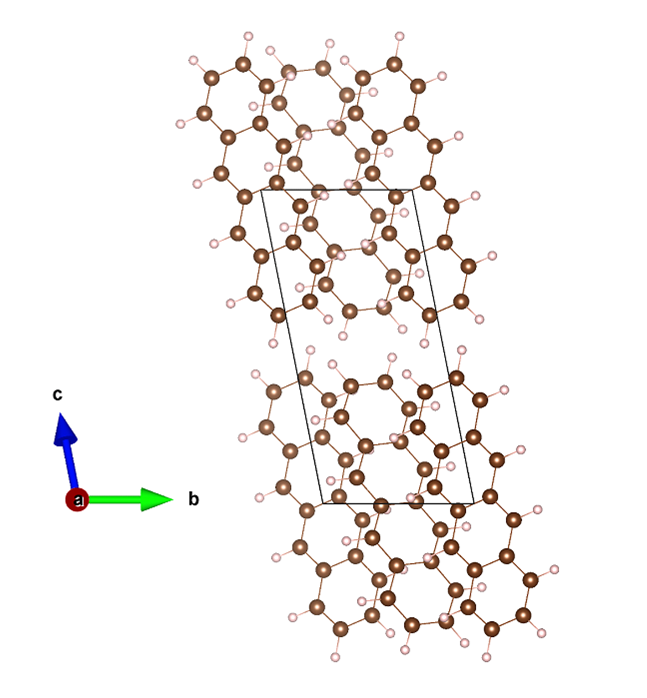
\includegraphics[scale=0.6]{T-a}
 		\caption{The \textit{bc} plane of Tetracene Crystal}  
 	\end{figure}
 	
 	\begin{figure}[h]
 		\centering
 		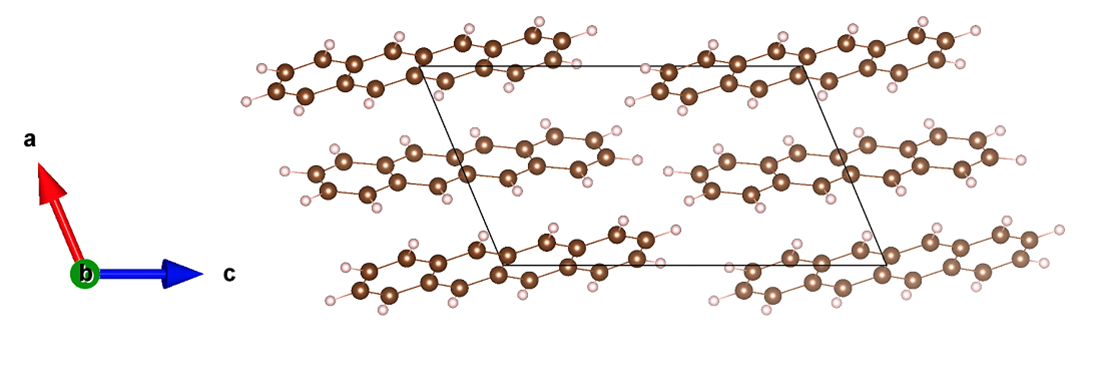
\includegraphics[scale=0.6]{T-b}
 		\caption{The \textit{ac} plane of Tetracene Crystal} 
 	\end{figure}
 	
 	\begin{figure}[h]
 		\centering
 		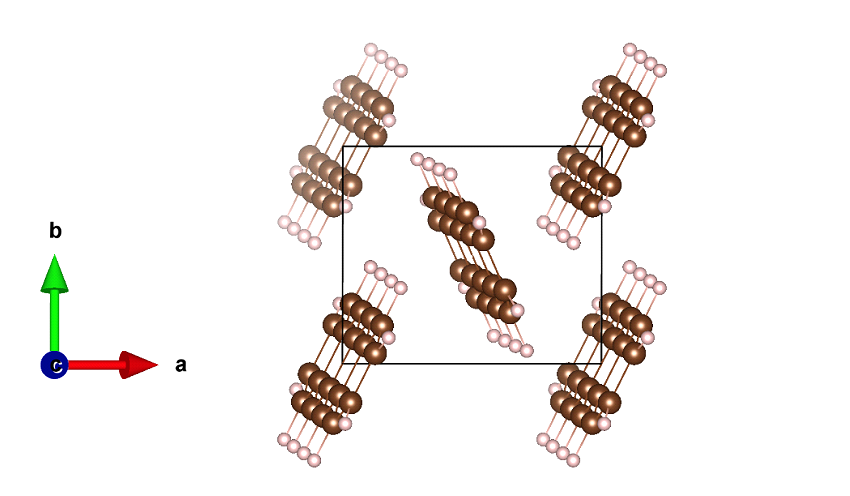
\includegraphics[scale=0.6]{T-c}
 		\caption{The \textit{ab} plane of Tetracene Crystal}  
 	\end{figure}
	
	
	
	 \begin{table}[h]
	 	\singlespacing
	 	\caption{ Calculated vibrational frequencies (cm$^{-1}$) of the monomer, dimer and solid-state (PBE tetracene system).} \label{table14}
	 	\begin{center}
	 		\begin{threeparttable}
	 			\begin{tabular}{c c c c c}
	 				\toprule
	 				\multicolumn{2}{p{4.5cm}}{\centering \textbf{Monomer}} & \textbf{Dimer} & \multicolumn{1}{p{4cm}}{\centering \textbf{Experimental} \\ \textbf{(P.A.) this work}} & \textbf{VASP/CRYSTAL}\\
	 				Assignment & $\nu$(cm$^{-1}$) & $\nu$(cm$^{-1}$) & $\nu$(cm$^{-1}$) & $\omega$(cm$^{-1}$) \\
	 				& Int(km/mol) & Int(km/mol) & & Int(relative) \\
	 				\midrule
	 				& & \textit{15 (<0.01)} & & \\
	 				& & \textit{31 (0)} & & \\
	 				& & \textit{52 (0)} & & \\
	 				$\nu_{1}$& 57 (0.8) & 59 (0.6) &  & 69.7 (8.2) \\
	 				& & \textit{80 (1.0)} & & \\
	 				& & \textit{87 (0.1)} & & \\
	 				& & 94 (0) & & \\
	 				& & 112 (0) & & \\
	 				$\nu_{2}$ & 93 (0) & 117 (0.3) & 106 (m) + sh & \multicolumn{1}{p{4cm}}{\centering 102.4 (2.1) \\ \textit{105.7 (9.5)}}\\
	 				& & 124 (0) & & \\
	 				3$\nu_{1}$& 132 (<0.01) & & & \\
	 				$\nu_{3}$& 153 (0.01) &  & 142 (m) & \multicolumn{1}{p{4cm}}{\centering 128.5 (7.1) \\ 148 (0.1)}\\ 
	 				& & 162 (0)&  & \\
	 				$\nu_{4}$& 164 (1.3) & 168 (1.7) & 166 (s) + sh & 164.6 (15.5) \\
	 				& & 169 (0) & & \\
	 				$\nu_{5}$ & 199 (0.05) & 176 (0.2) & 197 (w) & 170.1 (0.1) \\
	 				$\nu_{1}+\nu_{3}$ & 201 (<0.01) &  &  & \\
	 				& & 208 (0) & & \\
	 				&  & 212 (0.09) & 217 (w) & \\
	 				$\nu_{1}+ 2\nu_{2}$ & 228 (<0.01) & & & \\
	 				$\nu_{2}+\nu_{3}$& 247 (0.01) &  & 252 (vw) & \\
	 				$\nu_{6}$ & 275 (1.03) & 282 (1.6) & 271 (m) & 267.4 (3.0)\\
	 				&  & 286 (0) &  & 274.6 (2.6)\\
	 				$\nu_{2}+ \nu_{5}$ & 293 (<0.01) &  & 306 (vw) & \\
	 				& & 316 (0) & & \\
	 				& & 316 (0.03) & & \\
	 				&  & 324 (0) & 322 (w) & 320.8 (0.9)\\
	 				$\nu_{8}$& 322 (<0.01) & 325 (0.06) & & 323.8 (0.5)\\
	 				&  & 335 (0.03) & 342 (w) & \\
	 				& & 335 (0) & & \\
	 				$\nu_{1}+ 2\nu_{3}$ & 353 (<0.01) & &  & \\	
	 				$\nu_{1}+ \nu_{8}$ & 379 (<0.01) & & & \\
	 				$\nu_{10}$ & 385 (0.04) & 390 (0.02) &  392 (w) & \\
	 				2$\nu_{1}+ \nu_{6}$ & 380 (<0.01) &  & & \\
	 				\bottomrule	    
	 			\end{tabular}
	 			
	 			\begin{tablenotes}
	 				\item[] Italic: Intermolecular modes
	 			\end{tablenotes}
	 		\end{threeparttable}
	 	\end{center}
	 \end{table}
	 
	 
	
	
	
\end{document}